% Resumen del proyecto para preparar la presentación (Grupo 3, MAPF, UdeSA)
% Compilar con: latexmk -xelatex resumen.tex
\documentclass[11pt,a4paper]{article}

\usepackage{fontspec}
\usepackage{unicode-math}
\setmainfont{Caladea}
\setsansfont{Inter}[BoldFont={Inter SemiBold}]
\setmonofont{DejaVu Sans Mono}[Scale=0.84]
\setmathfont{Latin Modern Math}
\usepackage{polyglossia}
\setdefaultlanguage{spanish}

\usepackage[margin=2.3cm,top=2.4cm,bottom=2.4cm]{geometry}
\usepackage{xcolor}
\usepackage{graphicx}
\usepackage{booktabs}
\usepackage{tabularx}
\usepackage{array}
\usepackage{colortbl}
\usepackage{enumitem}
\usepackage{titlesec}
\usepackage{fancyhdr}
\usepackage{caption}
\usepackage[most]{tcolorbox}
\usepackage{tikz}
\usetikzlibrary{arrows.meta,positioning,shapes.geometric,calc,fit,backgrounds}
\usepackage{multicol}
\usepackage{amsmath}
\usepackage{microtype}
\usepackage[hidelinks]{hyperref}

% ---------------------------------------------------------------- colores
\definecolor{ink}{HTML}{0B0B0B}
\definecolor{ink2}{HTML}{52514E}
\definecolor{muted}{HTML}{8A8984}
\definecolor{grid}{HTML}{E6E5DF}
\definecolor{paper}{HTML}{F6F5F1}
\definecolor{crr}{HTML}{2A78D6}
\definecolor{bsm}{HTML}{EB6834}
\definecolor{aqua}{HTML}{1BAF7A}
\definecolor{amber}{HTML}{EDA100}
\definecolor{alert}{HTML}{E34948}
\definecolor{violet}{HTML}{6250D6}
\definecolor{navy}{HTML}{14213D}

% ---------------------------------------------------------------- tipografía de títulos
\titleformat{\section}{\sffamily\bfseries\LARGE\color{navy}}{\color{crr}\thesection}{0.6em}{}[\vspace{-0.4em}{\color{crr}\rule{\linewidth}{1.2pt}}]
\titleformat{\subsection}{\sffamily\bfseries\large\color{navy}}{\color{crr}\thesubsection}{0.5em}{}
\titleformat{\subsubsection}{\sffamily\bfseries\normalsize\color{ink}}{}{0em}{}
\titlespacing*{\section}{0pt}{1.4em}{1.0em}
\titlespacing*{\subsection}{0pt}{1.2em}{0.5em}
\setlength{\parindent}{0pt}
\setlength{\parskip}{0.55em}
\linespread{1.08}
\setlength{\emergencystretch}{3em}

\captionsetup{font={small,sf},labelfont={bf,color=navy},textfont={color=ink2},skip=4pt}
\setlist{itemsep=0.25em,topsep=0.3em,leftmargin=1.4em}

\pagestyle{fancy}
\fancyhf{}
\renewcommand{\headrulewidth}{0pt}
\fancyhead[L]{\sffamily\scriptsize\color{muted}Grupo 3 · Opciones sobre Defensa (RTX, BA, LMT)}
\fancyhead[R]{\sffamily\scriptsize\color{muted}Resumen para la presentación}
\fancyfoot[C]{\sffamily\small\color{ink2}\thepage}

% ---------------------------------------------------------------- cajas
\newtcolorbox{idea}[1][]{enhanced,colback=crr!6,colframe=crr,boxrule=0pt,leftrule=3pt,arc=1pt,
  left=8pt,right=8pt,top=5pt,bottom=5pt,fonttitle=\sffamily\bfseries\small,coltitle=crr,
  title={#1},attach title to upper={\par\vspace{2pt}},before skip=8pt,after skip=8pt}
\newtcolorbox{criollo}[1][En criollo]{enhanced,colback=aqua!7,colframe=aqua,boxrule=0pt,leftrule=3pt,arc=1pt,
  left=8pt,right=8pt,top=5pt,bottom=5pt,fonttitle=\sffamily\bfseries\small,coltitle=aqua!70!black,
  title={#1},attach title to upper={\par\vspace{2pt}},before skip=8pt,after skip=8pt}
\newtcolorbox{ojo}[1][Ojo]{enhanced,colback=amber!8,colframe=amber,boxrule=0pt,leftrule=3pt,arc=1pt,
  left=8pt,right=8pt,top=5pt,bottom=5pt,fonttitle=\sffamily\bfseries\small,coltitle=amber!70!black,
  title={#1},attach title to upper={\par\vspace{2pt}},before skip=8pt,after skip=8pt}
\newtcolorbox{formula}{enhanced,colback=paper,colframe=paper,arc=2pt,left=10pt,right=10pt,top=4pt,bottom=4pt,
  before skip=6pt,after skip=6pt}

% Tarjeta de corrección: título, qué estaba mal, por qué importaba, qué hicimos
\newcommand{\correccion}[4]{%
\begin{tcolorbox}[enhanced,colback=white,colframe=grid,boxrule=0.8pt,arc=3pt,left=9pt,right=9pt,top=6pt,bottom=6pt,
  title={\sffamily\bfseries #1},colbacktitle=navy,coltitle=white,fonttitle=\sffamily\bfseries\small,before skip=7pt,after skip=7pt]
{\sffamily\small\bfseries\color{alert}Qué estaba mal.}\ #2\par\vspace{3pt}
{\sffamily\small\bfseries\color{amber!80!black}Por qué importaba.}\ #3\par\vspace{3pt}
{\sffamily\small\bfseries\color{aqua!70!black}Qué hicimos.}\ #4
\end{tcolorbox}}

% Ficha de número grande
\newcommand{\kpi}[3]{%
\begin{tcolorbox}[enhanced,colback=paper,colframe=paper,arc=3pt,width=\linewidth,halign=center,valign=center,
  height=2.55cm,left=4pt,right=4pt,top=4pt,bottom=4pt]
{\sffamily\bfseries\fontsize{19}{21}\selectfont\color{#3}#1}\par\vspace{3pt}
{\sffamily\footnotesize\color{ink2}#2}
\end{tcolorbox}}

\newcommand{\code}[1]{\texttt{\detokenize{#1}}}
\newcommand{\usd}[1]{USD~#1}
\newcommand{\crrname}{\textcolor{crr}{\textbf{binomial (CRR)}}}
\newcommand{\bsname}{\textcolor{bsm}{\textbf{Black-Scholes}}}

\begin{document}

% ================================================================ PORTADA
\begin{titlepage}
\begin{tikzpicture}[remember picture,overlay]
  \fill[navy] (current page.north west) rectangle ([yshift=-10.5cm]current page.north east);
  \fill[crr] ([yshift=-10.5cm]current page.north west) rectangle ([yshift=-10.75cm]current page.north east);
  \node[anchor=north west,text width=16cm,align=left] at ([xshift=2.3cm,yshift=-2.4cm]current page.north west)
   {\sffamily\color{white!70!crr}\large MAPF · Universidad de San Andrés · Trabajo Práctico};
  \node[anchor=north west,text width=16.5cm,align=left] at ([xshift=2.3cm,yshift=-3.5cm]current page.north west)
   {\sffamily\bfseries\color{white}\fontsize{30}{35}\selectfont Opciones sobre Defensa:\\[2pt] del arbitraje a un sistema\\[2pt] que opera solo};
  \node[anchor=north west,text width=16cm,align=left] at ([xshift=2.3cm,yshift=-7.9cm]current page.north west)
   {\sffamily\color{white!85!crr}\Large Resumen completo del proyecto para armar la presentación};
\end{tikzpicture}
\vspace*{10.2cm}

{\sffamily\color{ink2}
\begin{tabularx}{\linewidth}{@{}lX@{}}
\textbf{Grupo 3} & A. Herrera, O. Lacunza, C. Grunewald, D. González y T. Brisighelli\\[3pt]
\textbf{Subyacentes} & RTX, BA y LMT (acciones del ETF ITA, sector Defensa de EE.\,UU.)\\[3pt]
\textbf{Fecha} & 23 de noviembre de 2026\\
\end{tabularx}}

\vspace{1.3cm}
\begin{minipage}[t]{0.31\linewidth}\kpi{7 años}{de historia simulada\\(2020–2026)}{crr}\end{minipage}\hfill
\begin{minipage}[t]{0.31\linewidth}\kpi{503.711}{cotizaciones reales\\de opciones}{bsm}\end{minipage}\hfill
\begin{minipage}[t]{0.31\linewidth}\kpi{184 tests}{automáticos que\\verifican el código}{aqua}\end{minipage}

\vfill
{\sffamily\small\color{ink2}
\textbf{Cómo leer este documento.} La sección 1 resume todo en una página. Las secciones 2 a 4 explican qué hace el
sistema y cómo calcula cada cosa. La 5 compara con la Parte 1 y la 6 cuenta, en lenguaje simple, todo lo que
corregimos. Las secciones 7 y 8 traen los resultados: la competencia entre modelos y la simulación histórica 2020–2026.
Al final están dónde corre el sistema, las limitaciones, las preguntas probables con su respuesta, un glosario y las
fuentes. Todos los números salen de archivos del repositorio y se pueden reproducir.}
\end{titlepage}

\tableofcontents
\thispagestyle{fancy}
\newpage

% ================================================================ 1. RESUMEN EJECUTIVO
\section{Resumen ejecutivo}

\begin{multicols}{2}
\begin{idea}[1 · Construimos un sistema completo]
Baja datos de opciones, calcula precios teóricos con \textbf{dos modelos} (binomial y Black-Scholes), detecta
estructuras mal valuadas, manda órdenes reales a una cuenta de prueba de Alpaca, cubre el riesgo con griegas y se
protege con reglas de corte. Corre solo, todos los días, en un servidor gratuito.
\end{idea}

\begin{idea}[2 · El arbitraje de la Parte 1 era un espejismo]
La entrega parcial mostraba \usd{19.055} de ganancia con 97,8\% de acierto. Con precios de compra y venta
\textbf{reales} y sincronizados, las 1.744 oportunidades de paridad bajan a 3 y \textbf{ninguna se puede ejecutar}.
\end{idea}

\begin{idea}[3 · El binomial valúa mejor, pero por poco]
Sobre 36.515 contratos, el árbol erra menos que Black-Scholes con altísima significancia ($DM^*=13{,}1$), y justo
donde dice la teoría: puts dentro del dinero y opciones con fecha de dividendo. Pero la diferencia supera medio
spread sólo en el 0,3\% de los casos.
\end{idea}

\begin{idea}[4 · La cobertura que conviene es la delta]
Cubrir la delta con acciones elimina el 95\% de la varianza diaria por \usd{3} por posición. Cubrir también la
gamma con opciones gana un punto antes de costos y pierde 16 después.
\end{idea}

\begin{idea}[5 · En siete años, la estrategia pierde siempre]
La simulación histórica del sistema completo (2020–2026) cierra 185 estructuras y pierde unos \usd{100} por
estructura, todos los años y con los dos modelos. La razón es la \textbf{selección adversa}: la orden se llena
justo cuando el modelo está desactualizado.
\end{idea}

\begin{idea}[6 · Decisión]
Con criterios escritos antes de ver el paper: \textbf{binomial y cobertura delta}. La ventaja del binomial es
estadística más que económica, y la simulación histórica no encuentra diferencia de P\&L entre modelos.
\end{idea}
\end{multicols}

\newpage
\subsection*{Los números para recordar}

\begin{minipage}[t]{0.235\linewidth}\kpi{1.744\,→\,0}{arbitrajes de paridad\\tras corregir datos}{alert}\end{minipage}\hfill
\begin{minipage}[t]{0.235\linewidth}\kpi{98\%}{precios del binomial\\dentro del bid-ask}{crr}\end{minipage}\hfill
\begin{minipage}[t]{0.235\linewidth}\kpi{95\%}{riesgo eliminado\\con cobertura delta}{aqua}\end{minipage}\hfill
\begin{minipage}[t]{0.235\linewidth}\kpi{6\%}{de las órdenes\\se llenan}{bsm}\end{minipage}

\vspace{4pt}
\begin{minipage}[t]{0.235\linewidth}\kpi{+11 / −100}{USD por estructura:\\prometido vs. real}{alert}\end{minipage}\hfill
\begin{minipage}[t]{0.235\linewidth}\kpi{$z=-0{,}21$}{CRR vs. BS en P\&L:\\sin diferencia}{violet}\end{minipage}\hfill
\begin{minipage}[t]{0.235\linewidth}\kpi{\usd{708}}{costo de cerrar todo:\\más que cualquier crisis}{amber!85!black}\end{minipage}\hfill
\begin{minipage}[t]{0.235\linewidth}\kpi{USD 0}{costo del servidor\\(Oracle Always Free)}{aqua}\end{minipage}

\begin{criollo}[La historia en tres frases]
Arrancamos buscando arbitrajes y descubrimos que los que encontrábamos eran errores de datos. Entonces construimos
una estrategia que apuesta a que el modelo tiene razón y la pusimos a competir con dos modelos distintos, con
coberturas y controles de riesgo de verdad. Siete años de historia muestran que el mercado de estas opciones es
eficiente: los modelos valúan bien, pero eso no alcanza para ganar plata pagando el spread.
\end{criollo}

\newpage
% ================================================================ 2. QUÉ HACE
\section{Qué hace el sistema}

El proyecto es un paquete de Python (\code{ita_options}) de unas \textbf{12.650 líneas} más 3.136 de tests. Hace
todo el recorrido que haría una mesa de opciones chica: mirar el mercado, decidir, operar, cubrirse, controlar el
riesgo y dejar registro. El universo son las opciones listadas de tres acciones del ETF ITA:
\textbf{RTX} (Raytheon), \textbf{BA} (Boeing) y \textbf{LMT} (Lockheed Martin).

\begin{figure}[h]
\centering
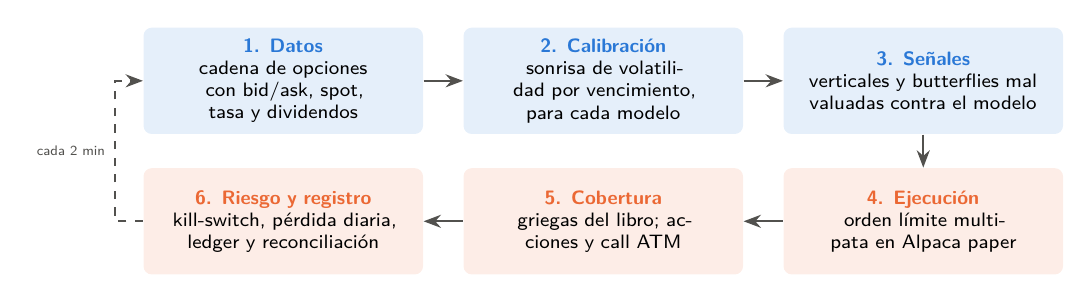
\begin{tikzpicture}[
  node distance=0.42cm and 0.5cm,
  box/.style={draw=none,fill=#1!12,rounded corners=3pt,minimum width=3.55cm,minimum height=1.35cm,
              text width=3.3cm,align=center,font=\sffamily\scriptsize},
  head/.style={font=\sffamily\bfseries\footnotesize},
  arr/.style={-{Stealth[length=2.2mm]},thick,color=ink2}]
\node[box=crr] (d) {{\color{crr}\bfseries 1. Datos}\\ cadena de opciones con bid/ask, spot, tasa y dividendos};
\node[box=crr,right=of d] (c) {{\color{crr}\bfseries 2. Calibración}\\ sonrisa de volatilidad por vencimiento, para cada modelo};
\node[box=crr,right=of c] (s) {{\color{crr}\bfseries 3. Señales}\\ verticales y butterflies mal valuadas contra el modelo};
\node[box=bsm,below=of s] (e) {{\color{bsm}\bfseries 4. Ejecución}\\ orden límite multipata en Alpaca paper};
\node[box=bsm,left=of e] (h) {{\color{bsm}\bfseries 5. Cobertura}\\ griegas del libro; acciones y call ATM};
\node[box=bsm,left=of h] (r) {{\color{bsm}\bfseries 6. Riesgo y registro}\\ kill-switch, pérdida diaria, ledger y reconciliación};
\draw[arr] (d) -- (c);
\draw[arr] (c) -- (s);
\draw[arr] (s) -- (e);
\draw[arr] (e) -- (h);
\draw[arr] (h) -- (r);
\draw[arr,dashed] (r.west) -- ++(-0.35,0) |- node[pos=0.25,left,font=\sffamily\tiny,text=ink2]{cada 2 min} (d.west);
\end{tikzpicture}
\caption{El ciclo que corre cada 120 segundos durante la rueda.}
\end{figure}

\subsection{El ciclo, paso a paso}

\begin{enumerate}[label=\textbf{\arabic*.}]
\item \textbf{Datos.} Pide a Alpaca el spot, el universo de contratos y las cotizaciones (bid y ask) de los tres
  subyacentes. Arma la cadena y descarta lo que no se puede operar: spread mayor a 25\% del precio, bid nulo,
  cotizaciones cruzadas o muy viejas.
\item \textbf{Calibración.} Cada modelo ajusta \emph{su propia} sonrisa de volatilidad por vencimiento con las
  opciones fuera del dinero (sección 4.4).
\item \textbf{Señales.} Con esa sonrisa valúa todas las verticales (comprar un strike y vender el siguiente) y
  butterflies (1, −2, 1) cerca del dinero, de 21 a 75 días. Si el mercado se aparta lo suficiente del modelo,
  propone una orden.
\item \textbf{Ejecución.} Manda una orden \emph{multipata límite} (todas las patas juntas, a un precio neto) que
  espera hasta 180 segundos y se cancela si no se llena.
\item \textbf{Cobertura.} Suma las griegas de las posiciones de cada modelo y subyacente y rebalancea con acciones
  y, si hace falta, con la call ATM más corta.
\item \textbf{Riesgo y registro.} Marca cada posición, aplica los cortes, compara su registro (una base SQLite) con
  lo que dice el broker y guarda todo para el reporte de la sesión.
\end{enumerate}

\begin{criollo}
Es un ``trader robot'' con dos cerebros: uno piensa con el modelo binomial y otro con Black-Scholes. Los dos miran el
mismo mercado, cada uno decide qué le parece barato o caro, operan en la misma cuenta y al final comparamos cuál
lo hizo mejor. Mientras tanto, un tercer componente se ocupa de que ninguno de los dos se exponga de más.
\end{criollo}

\newpage
% ================================================================ 3. CAPACIDADES
\section{De qué es capaz}

\subsection{Modos de uso}

\begin{center}
\small
\begin{tabularx}{\linewidth}{@{}>{\sffamily\bfseries\raggedright\arraybackslash\leavevmode\color{navy}}p{3.2cm}X>{\ttfamily\scriptsize}p{4.2cm}@{}}
\toprule
\normalfont\sffamily\bfseries Modo & \sffamily\bfseries Qué hace & \normalfont\sffamily\bfseries Dónde \\
\midrule
Paper trading en vivo & Opera la cuenta de prueba de Alpaca durante toda la rueda, con los dos modelos compitiendo y coberturas. & paper-run --live \\
Prueba en seco & Mismo ciclo, sin mandar órdenes: verifica conexión, claves y datos. & paper-run \\
Diagnóstico & Revisa autenticación, permisos de opciones y datos en vivo. & doctor \\
Detectores de arbitraje & Cinco detectores \emph{model-free}: monotonicidad, cota vertical, butterfly, paridad put-call y calendario. & arbitrage.py \\
Backtest de la Parte 1 & Arbitraje con carry y valor relativo con walk-forward. & backtest.py, rv\_backtest.py \\
Comparación de modelos & Binomial contra Black-Scholes sobre 36.515 contratos, con Diebold-Mariano. & run\_model\_comparison.py \\
Backtest de coberturas & Cinco estrategias con griegas sobre 3.272 días-posición. & run\_hedging.py \\
Estrés Monte Carlo & GBM, Heston y Merton correlacionados, más escenarios históricos. & run\_stress.py \\
Simulación histórica & El sistema completo, foto por foto, de 2020 a 2026. & run\_replay.py \\
Tabla de decisión & Aplica los criterios fijados de antemano y elige modelo y cobertura. & scorecard.py \\
\bottomrule
\end{tabularx}
\end{center}

\subsection{Reglas de producción}

\begin{center}
\small
\begin{tabularx}{0.86\linewidth}{@{}>{\sffamily}lX@{}}
\toprule
\textbf{Parámetro} & \textbf{Valor} \\
\midrule
Estructuras & verticales y butterflies (pérdida máxima acotada) \\
Tamaño & 1 unidad por estructura \\
Vencimientos & de 21 a 75 días \\
Edge mínimo contra el modelo & \usd{10} neto de comisiones \\
Cupo & 3 estructuras abiertas por modelo, 6 en total \\
Take-profit & cuando la ganancia, pagando el spread de salida, llega al 60\% del edge \\
Kill-switch & pérdida de \usd{250} por estructura, medida al mid \\
Pérdida diaria máxima & \usd{1.000} en toda la cuenta, al mid y con la cobertura incluida \\
Cierre anticipado & 2 días antes del vencimiento \\
Cobertura & delta-gamma entera: banda de 10 acciones, hasta 5 contratos de la call ATM \\
Corte manual & crear un archivo \code{KILL} cierra todo en el ciclo siguiente \\
Frecuencia & un ciclo cada 120 segundos \\
\bottomrule
\end{tabularx}
\end{center}

\subsection{Calidad y reproducibilidad}

\begin{itemize}
\item \textbf{184 tests automáticos}: verifican, por ejemplo, que el árbol reproduzca el ejemplo del Hull
  (\usd{4,4404} contra 4,44), que los detectores no encuentren nada en cadenas sin arbitraje por construcción, o que
  el kill-switch no se dispare al abrir una posición.
\item \textbf{Sin lookahead}: la señal de una foto se ejecuta contra la foto siguiente; los dividendos entran recién
  cuando se declaran.
\item \textbf{Mismo código en vivo y en backtest}: verificamos que, sobre la misma cadena, los dos caminos den el
  mismo valor (diferencia máxima 0).
\item \textbf{Todo reproducible}: cada número de este documento sale de un script del repositorio.
\end{itemize}

% ================================================================ 4. CÓMO CALCULA
\section{Cómo calcula cada cosa}

\subsection{El dividendo: modelo \emph{escrowed}}

RTX y LMT pagan dividendos trimestrales (LMT, \usd{3,45} por acción). BA no paga desde 2020. El dividendo hace caer
la acción en la fecha ex, así que hay que descontarlo. Usamos el modelo \emph{escrowed} (Hull, cap.~21): el precio se
separa en una parte riesgosa $S^*$ y el valor presente de los dividendos que faltan cobrar,

\begin{formula}
\[
S_t = S^*_t + D(t), \qquad D(t) = \sum_{t < t_i \le T} d_i\, e^{-r(t_i - t)} .
\]
\end{formula}

La volatilidad se aplica sólo a $S^*$. Los dividendos son \textbf{point-in-time}: en cada fecha se usan sólo los ya
declarados y, más allá, se repite el último monto cada 91 días.

\begin{criollo}
El dividendo no es ``un poquito de rendimiento todos los días'': es un pago grande en una fecha precisa. Si el
modelo no sabe en qué día cae, valúa mal justo las opciones que más dependen de él.
\end{criollo}

\subsection{Black-Scholes}

Fórmula europea (sólo se ejerce al vencimiento) aplicada sobre $S^* = S - D(0)$:

\begin{formula}
\[
C = S^* N(d_1) - K e^{-r\tau} N(d_2), \qquad P = K e^{-r\tau} N(-d_2) - S^* N(-d_1),
\]
\[
d_{1,2} = \frac{\ln(S^*/K) + (r \pm \tfrac12\sigma^2)\tau}{\sigma\sqrt\tau}.
\]
\end{formula}

\subsection{Binomial de Cox-Ross-Rubinstein}

El árbol divide el plazo en $N=100$ pasos de $\Delta t = \tau/N$. En cada paso la acción sube o baja:

\begin{formula}
\[
u = e^{\sigma\sqrt{\Delta t}}, \qquad d = \frac1u, \qquad p = \frac{e^{r\Delta t} - d}{u - d},
\]
\[
V_j^n = \max\Big(\underbrace{\Psi\big(S^*_{n,j} + D(t_n)\big)}_{\text{ejercer hoy}},\;
\underbrace{e^{-r\Delta t}\big[p\,V^{n+1}_{j+1} + (1-p)\,V^{n+1}_j\big]}_{\text{esperar}}\Big).
\]
\end{formula}

La diferencia clave con Black-Scholes es el $\max$: en cada nodo el árbol compara ejercer ya contra esperar. Eso es
lo que vale una opción \textbf{americana}, y las opciones sobre acciones de EE.\,UU. son americanas.

\begin{figure}[h]
\centering
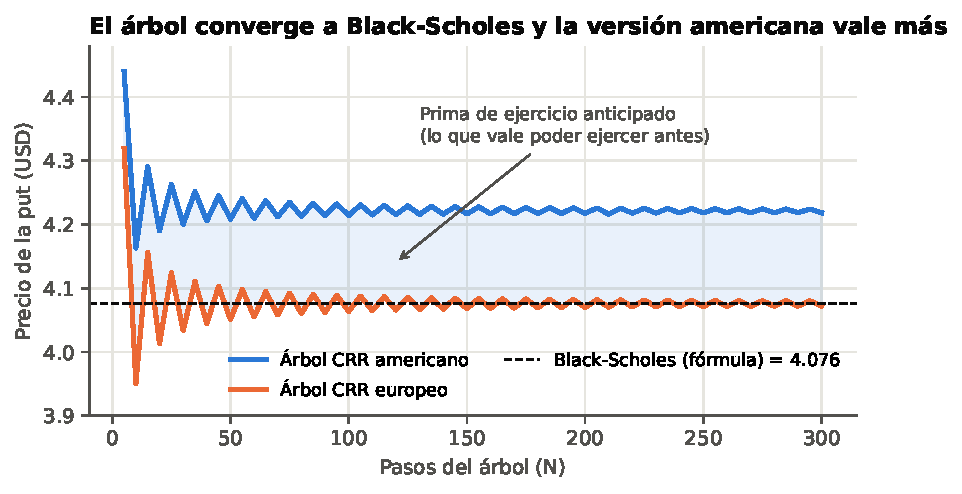
\includegraphics[width=0.86\linewidth]{figs/f01_convergencia.pdf}
\caption{Put del ejemplo del Hull ($S=52$, $K=50$, $r=10\%$, $\sigma=40\%$, 5 meses, dividendo de \usd{2,06}). La
versión europea del árbol converge a la fórmula de Black-Scholes; la americana vale más, y esa diferencia es la
\emph{prima de ejercicio anticipado}.}
\end{figure}

\textbf{Prima de ejercicio anticipado (EEP).} Se mide con el mismo árbol, con y sin la opción de ejercer:
$\mathrm{EEP} = V^{CRR}_{\text{am}} - V^{CRR}_{\text{eu}} \ge 0$. Según la teoría aparece en las \textbf{puts dentro
del dinero} y en los \textbf{calls justo antes de una fecha ex}; sin dividendos, un call americano vale lo mismo que
uno europeo (Merton, 1973).

\subsection{Volatilidad implícita y sonrisa}

La volatilidad implícita (IV) es la $\sigma$ que hace que el modelo dé el precio de mercado. Se invierte con el
método de Newton desde la IV de Black-Scholes y, si no converge, con Brent. Pero invertir contrato por contrato
reproduce cada precio por construcción y no dice nada. Lo que importa es \textbf{calibrar una superficie} con pocos
parámetros, por vencimiento:

\begin{formula}
\[
\sigma(k) = a + b\,k + c\,k^2, \qquad k = \ln\frac{K}{F},
\]
\end{formula}

ajustada por mínimos cuadrados ponderados por vega y por la inversa del spread, sólo con las opciones fuera del
dinero (las más líquidas y sin prima de ejercicio). \textbf{Cada modelo ajusta su sonrisa con sus propios precios}:
así cada uno compite con su mejor versión.

\begin{figure}[h]
\centering
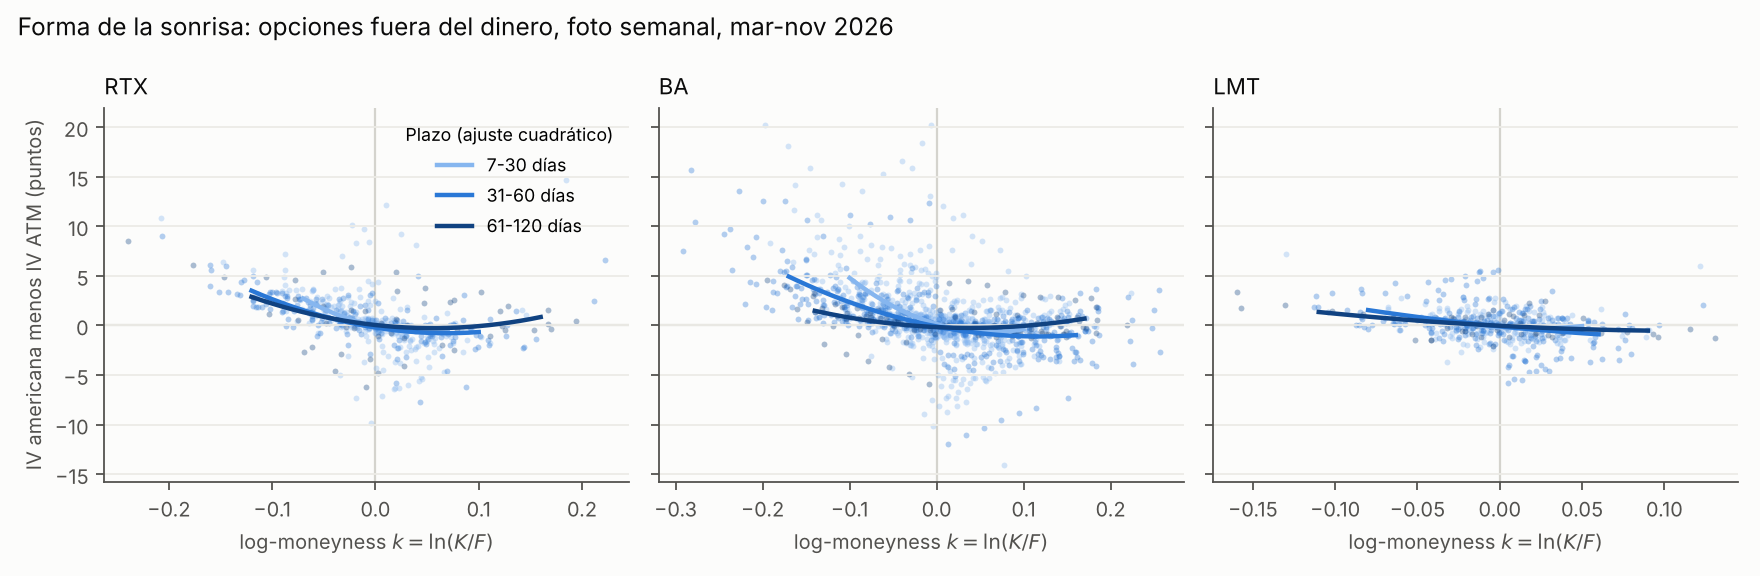
\includegraphics[width=0.72\linewidth]{../reportes_dolthub/iv_vs_moneyness.png}
\caption{Forma de la sonrisa en 2026: las puts fuera del dinero (izquierda) cotizan con más volatilidad que las
calls. Es el \emph{skew} típico de acciones, más marcado en BA.}
\end{figure}

\begin{figure}[h]
\centering
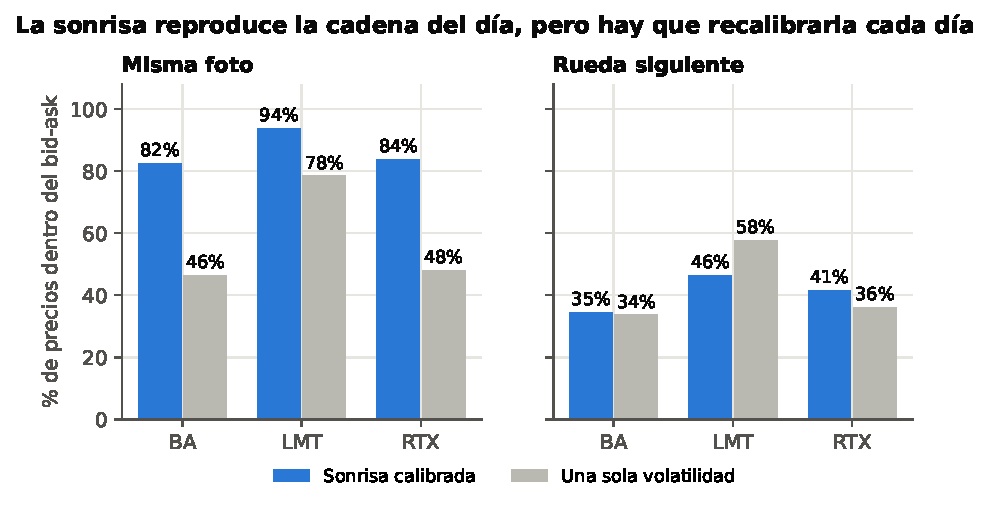
\includegraphics[width=0.92\linewidth]{figs/f03_calibracion.pdf}
\caption{Con la sonrisa, entre 82\% y 94\% de los precios caen dentro del bid-ask el mismo día, contra 46\% a 78\%
con una sola volatilidad. Al día siguiente la ventaja se pierde porque el \emph{nivel} de la volatilidad se mueve:
hay que recalibrar en cada foto, y el sistema lo hace.}
\end{figure}

\subsection{Spot implícito}

La foto de opciones y el cierre de la acción no son simultáneos. Por eso el spot se estima desde la propia cadena,
con la paridad put-call en los pares cercanos al dinero:

\begin{formula}
\[
\hat S_t = \operatorname{mediana}_{K \approx S}\left(C^{\text{mid}}_K - P^{\text{mid}}_K + K e^{-r\tau} + D\right).
\]
\end{formula}

En 2026 la brecha con el cierre tiene mediana 0,19\% y percentil 90 de 1,26\%: hay días en que la cadena cotiza
contra un spot varios dólares distinto. Con el spot implícito, el 98\% de los precios del modelo caen dentro del
bid-ask; con el cierre, sólo el 80\%.

\subsection{Griegas}

\begin{center}
\small
\begin{tabularx}{\linewidth}{@{}>{\sffamily\bfseries}l>{\centering\arraybackslash}p{2.7cm}X@{}}
\toprule
Griega & Definición & Qué mide \\
\midrule
Delta $\Delta$ & $\partial V/\partial S$ & cuánto cambia la opción si la acción sube \usd{1}; es la cantidad de acciones que replica la opción \\
Gamma $\Gamma$ & $\partial^2 V/\partial S^2$ & cuánto cambia la delta; mide la curvatura y cuánto hay que rebalancear \\
Vega $\mathcal V$ & $\partial V/\partial\sigma$ & sensibilidad a la volatilidad \\
Theta $\Theta$ & $\partial V/\partial t$ & cuánto valor pierde la opción con el paso del tiempo \\
Rho $\rho$ & $\partial V/\partial r$ & sensibilidad a la tasa \\
\bottomrule
\end{tabularx}
\end{center}

En Black-Scholes son fórmulas cerradas; con dividendo escrowed, $\rho$ y $\Theta$ llevan un término extra porque
$D$ depende de $r$ y de $t$: $\rho = \rho^* + \Delta \sum_i d_i t_i e^{-r t_i}$ y $\Theta = \Theta^* - \Delta\, r D$. En
el árbol, $\Delta$ y $\Gamma$ salen de los nodos de los pasos 1 y 2; $\mathcal V$ y $\rho$ por diferencias centrales,
promediando árboles de $N$ y $N+1$ pasos para cancelar la oscilación que se ve en la figura de convergencia.

\subsection{La señal: valor relativo contra el modelo}

Para cada vertical y butterfly con $V$ el valor del modelo, $m$ el margen pedido (edge mínimo más comisiones) y
$bid_{\text{neto}}$, $ask_{\text{neto}}$ lo que paga y cobra el mercado por la estructura entera, se publica una orden
límite \textbf{dentro} del spread:

\begin{formula}
\[
L_{\text{compra}} = V - m, \qquad L_{\text{venta}} = V + m, \qquad
\text{sólo si } bid_{\text{neto}} < L < ask_{\text{neto}},
\]
\[
\text{edge} = 100\,|V - L| - \text{comisiones} \ \ge\ \text{USD }10.
\]
\end{formula}

\begin{idea}[Ejemplo numérico]
Vertical de calls de BA 220/225. El modelo dice que vale \usd{2,50} por acción. El mercado la ofrece con
$bid_{\text{neto}} = 2{,}10$ y $ask_{\text{neto}} = 2{,}70$. Con dos patas, las comisiones son
$2 \times 0{,}65 = 1{,}30$ USD, y $m = (10 + 1{,}30)/100 = 0{,}113$. Se publica una compra a
$L = 2{,}50 - 0{,}113 = 2{,}387$, dentro del spread. Si se llena, se compró \usd{11,30} por debajo del modelo, que es
exactamente el edge pedido más las comisiones.
\end{idea}

Si los dos modelos proponen las mismas patas, se ejecuta una sola vez. Entre modelos la prioridad se alterna en cada
ciclo, y ninguno puede tener más de 3 estructuras abiertas.

\subsection{Cuándo se llena y cuándo se cierra}

\begin{itemize}
\item \textbf{Llenado en la simulación}: la orden publicada en una foto se llena en la foto siguiente \emph{sólo si}
  el mercado la cruza (el ask neto baja hasta $L$), y al precio $L$. Si no, se cancela.
\item \textbf{Take-profit}: se cierra cuando la ganancia \emph{después de pagar el spread de salida} llega al 60\% del
  edge. Se mide a liquidación porque esa plata tiene que poder cobrarse.
\item \textbf{Kill-switch}: se cierra si la pérdida, medida \textbf{al mid}, supera \usd{250}.
\item \textbf{Pérdida diaria}: si la cuenta entera (con la cobertura) pierde más de \usd{1.000} al mid, se cierra todo.
\item \textbf{Vencimiento}: se cierra 2 días antes; si llega a vencer, se liquida al valor intrínseco.
\end{itemize}

\subsection{Coberturas}

Para una posición de $q$ contratos de la opción $O$ y una opción de cobertura $H$:

\begin{formula}
\begin{align*}
\text{Delta (acciones):}\quad & h = -100\, q\, \Delta_O \\
\text{Delta-gamma:}\quad & n = -q\,\Gamma_O/\Gamma_H, \qquad h = -100\,(q\,\Delta_O + n\,\Delta_H) \\
\text{Delta-vega:}\quad & n = -q\,\mathcal V_O/\mathcal V_H \\
\text{Delta-gamma entera:}\quad & n = \max\big(\operatorname{round}(-q\,\Gamma_O/\Gamma_H),\,0\big)
\end{align*}
\end{formula}

La versión \emph{entera} es la que se puede ejecutar: contratos enteros y sólo compras, porque con el nivel 3 de
opciones de Alpaca no se puede vender una opción descubierta. En producción se cubre cada \emph{libro} (un modelo en
un subyacente) con las griegas de su propio modelo, y la delta se rebalancea sólo si se aparta 10 acciones o más del
objetivo, para no pagar costos por movimientos chicos (la idea de Leland, 1985).

\subsection{Cómo se comparan los modelos: Diebold-Mariano}

Para cada contrato, el error se mide en \emph{medios spreads}: $L = |\hat V - m|/(s/2)$, donde un valor menor a 1
significa que el precio del modelo cae dentro del bid-ask. Por día se promedia la diferencia de errores y se testea
si su media es cero:

\begin{formula}
\[
d_t = \frac{1}{n_t}\sum_{i \in t}\left(L^{BS}_i - L^{CRR}_i\right), \qquad
DM^* = \frac{\bar d}{\sqrt{\hat\Omega/T}}\sqrt{\frac{T-1}{T}},
\]
\end{formula}

con la varianza $\hat\Omega$ de Newey-West y la corrección de muestra chica de Harvey, Leybourne y Newbold.
$\bar d > 0$ significa que el binomial erra menos. Promediar dentro del día evita tratar como independientes contratos
que comparten el mismo shock.

\subsection{Efectividad de una cobertura y riesgo de cola}

\begin{formula}
\[
E = 1 - \frac{\operatorname{Var}(\Delta\Pi^{\text{cubierta}})}{\operatorname{Var}(\Delta\Pi^{\text{sin cubrir}})},
\qquad
\mathrm{ES}_{99\%} = -\,\mathbb E\big[\,\Pi \mid \Pi \le \mathrm{VaR}_{1\%}\big].
\]
\end{formula}

$E = 95\%$ quiere decir que la cobertura elimina el 95\% de la varianza diaria. El \emph{expected shortfall} al 99\%
es la pérdida promedio en el peor 1\% de los escenarios.

\subsection{Monte Carlo: tres formas de que el mundo se mueva}

Los tres subyacentes se simulan juntos, con shocks correlacionados por Cholesky ($Z = L\varepsilon$, $LL^\top =
\Sigma$, correlación de 5 años de retornos diarios):

\begin{itemize}
\item \textbf{GBM}: $d\ln S^* = (r - \tfrac12\sigma^2)\,dt + \sigma\,dW$, con la volatilidad implícita ATM del día.
\item \textbf{Heston}: la volatilidad también es aleatoria y vuelve a una media,
  $v_{k+1} = v_k + \kappa(\theta - v_k^+)\Delta t + \xi\sqrt{v_k^+\Delta t}\,Z^v$, calibrado con la IV ATM histórica
  (y una versión estresada con $\rho = -0{,}7$ y $\xi = 1$).
\item \textbf{Merton}: difusión más saltos, $d\ln S^* = (\ldots)\,dt + \sigma\,dW + J\,dN$. La versión
  \emph{sectorial} hace saltar a las tres acciones juntas (un shock de defensa: $-8\%$ cuatro veces por año).
\end{itemize}

Además se prueban escenarios determinísticos: caída de 15\% en un día con la volatilidad 15 puntos arriba, suba de
10\%, volatilidad +20 puntos, y la repetición de las 10 ruedas del COVID y de los aranceles de abril de 2025.

\newpage
% ================================================================ 5. PARTE 1 vs PARTE 2
\section{En qué se diferencia de la Parte 1}

\begin{center}
\small
\renewcommand{\arraystretch}{1.25}
\begin{tabularx}{\linewidth}{@{}>{\sffamily\bfseries\raggedright\arraybackslash\leavevmode\color{navy}}p{2.9cm}>{\raggedright\arraybackslash}X>{\raggedright\arraybackslash}X@{}}
\toprule
 & \sffamily\bfseries Entrega parcial (septiembre) & \sffamily\bfseries Hoy (Parte 2) \\
\midrule
Datos & bid y ask \textbf{sintéticos} alrededor de cierres no simultáneos & bid y ask \textbf{observados} (DoltHub): 181 ruedas en 2026 y 1.229 desde 2020 \\
Modelos & sólo binomial & binomial \textbf{y} Black-Scholes, compitiendo en la misma cuenta \\
Dividendos & yield continuo & dividendo discreto (\emph{escrowed}), declarado \emph{point-in-time} \\
Volatilidad & IV contrato por contrato & sonrisa calibrada por vencimiento, para cada modelo \\
Estrategia & arbitraje \emph{model-free} (paridad) & valor relativo en verticales y butterflies, con pérdida acotada \\
Resultado reportado & \usd{19.055}, 97,8\% de acierto & ninguna operación de arbitraje; la estrategia pierde y sabemos por qué \\
Validación & sin separación de muestras & walk-forward fuera de muestra, Sharpe deflactado, siete años de simulación \\
Coberturas & no había & delta, delta-gamma y delta-vega, en backtest y en vivo \\
Riesgo & kill-switch básico & kill-switch al mid, pérdida diaria, reconciliación con el broker, corte manual, estrés Monte Carlo \\
Ejecución & piloto manual & corre solo en un servidor gratuito, de lunes a viernes \\
Decisión & no había criterio formal & tabla de criterios fijados antes del paper \\
Tests & pocos & 184 \\
\bottomrule
\end{tabularx}
\end{center}

\begin{criollo}
En la Parte 1 teníamos un motor que encontraba plata fácil. En la Parte 2 descubrimos que esa plata era un error de
datos, armamos un sistema honesto y profesional, y lo pusimos a prueba contra siete años de mercado real. El
resultado es menos espectacular, pero es verdad, y está medido con el rigor que pide un trabajo cuantitativo.
\end{criollo}

\newpage
% ================================================================ 6. CORRECCIONES
\section{Las correcciones, en lenguaje simple}

Después de la Parte 1 recibimos una devolución con siete puntos y, revisando el código, encontramos varios errores
más. Cada tarjeta cuenta qué estaba mal, por qué importaba y qué hicimos.

\correccion{1 · Precios inventados}
{Los precios de compra y venta (bid y ask) de la Parte 1 eran \emph{sintéticos}: los armábamos alrededor de precios
de cierre que, además, no eran del mismo momento para la opción y para la acción.}
{Un arbitraje existe o no según el bid y el ask \emph{reales}. Con precios inventados, el sistema encontraba
``oportunidades'' que en el mercado no existían. Ahí salían los \usd{19.055} y el 97,8\% de acierto.}
{Descargamos los bid y ask reales de una base pública (DoltHub): 95.290 cotizaciones de 2026 y después 503.711 desde
2020. Con esos precios las operaciones de arbitraje \textbf{desaparecen}.}

\correccion{2 · El dividendo repartido en todos los días}
{Tratábamos el dividendo como un rendimiento continuo, como si la acción ``pagara un poquito'' todos los días.}
{En la realidad LMT paga \usd{3,45} de golpe en una fecha. Cerca de esa fecha, el modelo se equivocaba y el error
aparecía como arbitraje. Fue lo que disparó el kill-switch en la paridad de LMT en la entrega parcial.}
{Usamos el dividendo discreto (modelo \emph{escrowed}): el modelo sabe en qué día cae cada pago. Elimina el 41\% del
edge fantasma de LMT en las tres semanas previas a cada fecha ex.}

\correccion{3 · La foto y el cierre no son del mismo momento}
{La foto de opciones se toma durante la rueda, pero comparábamos contra el precio de cierre de la acción.}
{Si la acción se movió entre la foto y el cierre, la paridad put-call parece violada aunque no lo esté. La brecha
llega a 1,26\% en el 10\% de los días.}
{Estimamos el spot \emph{desde la propia cadena} (spot implícito) y exigimos que una violación supere ese desfase.
Las 1.744 violaciones de paridad bajan a 3, y ninguna se puede ejecutar al día siguiente.}

\begin{figure}[h]
\centering
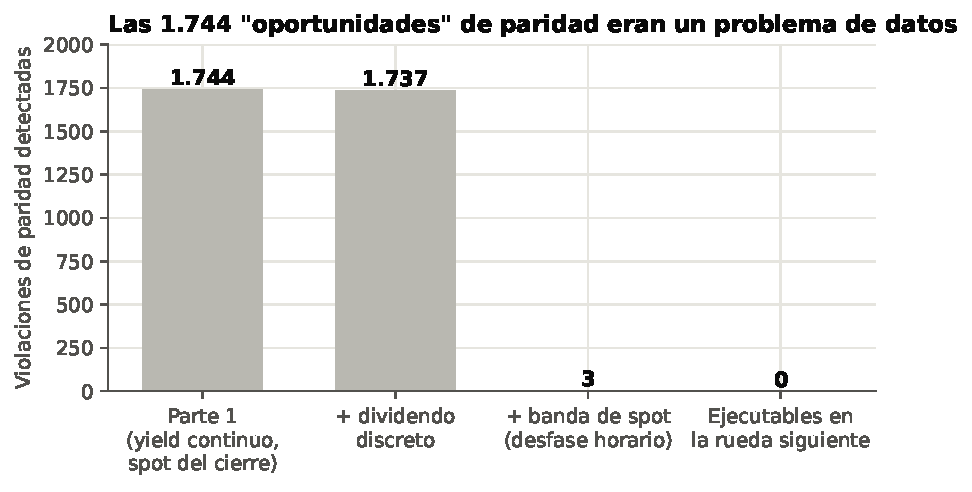
\includegraphics[width=0.84\linewidth]{figs/f02_paridad.pdf}
\caption{Cada corrección, aplicada en orden, sobre las 181 ruedas de 2026.}
\end{figure}

\correccion{4 · Un signo al revés}
{En la conversión reversa, el costo de pedir prestada la acción \emph{sumaba} al resultado en vez de restar, y el
medio spread de la acción tenía el signo invertido.}
{Inflaba justamente las operaciones de paridad, que eran el 87\% del P\&L de la entrega parcial.}
{Corregimos los signos y agregamos tests que fallan con la versión anterior.}

\correccion{5 · Sin prueba fuera de muestra}
{Elegíamos los parámetros mirando los mismos datos con los que medíamos el resultado.}
{Es la forma más común de engañarse: casi cualquier estrategia parece buena en los datos con los que se la ajustó.}
{\emph{Walk-forward}: calibramos con marzo–junio y evaluamos mes a mes de julio a noviembre, con la grilla de
parámetros declarada antes de mirar. Medimos con el \emph{Sharpe deflactado}, que descuenta cuántas configuraciones
probamos. Ninguna se distingue del ruido.}

\correccion{6 · Invertir no es calibrar}
{Sacábamos la volatilidad implícita de cada contrato por separado.}
{Eso reproduce cada precio por construcción: el error da cero y no prueba nada sobre el modelo.}
{Calibramos una \emph{sonrisa} de tres parámetros por vencimiento y medimos el error de revaluación dentro y fuera
de muestra (sección 4.4).}

\correccion{7 · Una estrategia que nunca operaba}
{Con datos reales no hay arbitraje, así que el paper trading se habría quedado sin posiciones.}
{La consigna pide comparar modelos en producción, y sin posiciones no hay nada que comparar.}
{Pasamos a una estrategia de \emph{valor relativo} contra el modelo, en verticales y butterflies (pérdida máxima
acotada), de 1 unidad. No es arbitraje y lo decimos: su edge depende de que el modelo tenga razón.}

\correccion{8 · El kill-switch que cortaba todo al abrir}
{El corte por pérdida se medía \emph{a liquidación}, es decir, como si hubiera que cerrar ya mismo cruzando el spread.}
{Una vertical de BA recién abierta ya ``pierde'' entre \usd{250} y 370 sólo por el spread: el kill-switch cerraba cada
posición en el mismo ciclo en que se abría. El backtest de la Parte 1 lo medía bien, pero el loop en vivo no, y
lo descubrió la prueba de estrés: con la regla vieja, el kill-switch saltaba en el 100\% de los escenarios.}
{El kill-switch y la pérdida diaria se miden \textbf{al mid}; el take-profit sigue a liquidación, porque esa ganancia
hay que poder cobrarla. Un test de regresión falla con la regla anterior.}

\correccion{9 · El dividendo continuo también sesgaba el ejercicio anticipado}
{Una primera versión del árbol usaba un ``yield equivalente'' para el dividendo.}
{Da bien el precio forward, pero reparte el dividendo en todo el plazo, y valúa mal el ejercicio del call justo antes
de la fecha ex: los calls dentro del dinero quedaban \usd{16} por contrato por debajo del mercado.}
{Comparamos los dos tratamientos sobre toda la cadena: el escrowed erra menos ($DM^* = 6{,}1$). Pasamos todo el
sistema (vivo, backtest y calibración) al escrowed y recalculamos la Parte 1, sin que cambie ninguna conclusión.}

\correccion{10 · El robot y el backtest no calculaban igual}
{En vivo la sonrisa se ajustaba también con contratos no operables y con 150 pasos de árbol; en el backtest, con
100 pasos y sólo contratos operables.}
{Si el backtest y la producción no hacen la misma cuenta, el backtest no predice nada de lo que va a pasar.}
{Unificamos el código y verificamos que, sobre la misma cadena, los dos caminos den exactamente el mismo valor.}

\correccion{11 · Errores en el material de clase}
{El notebook de la cátedra tenía la butterfly con el signo cambiado, el detector de calendario medía el spread, un
ask en cero se tomaba como una opción gratis, la tabla de griegas tenía la put con el signo cambiado, y el simulador
de Heston usaba la varianza inicial durante toda la trayectoria.}
{En Heston, por ejemplo, la volatilidad estocástica nunca le llegaba al precio: era un GBM disfrazado.}
{Lo corregimos en nuestro código y lo documentamos; cada corrección tiene su test.}

\correccion{12 · Monitorear es un proceso, no una foto}
{El piloto de paper de la Parte 1 mandaba órdenes y no seguía las posiciones.}
{En producción hay que saber en todo momento qué se tiene, cuánto se pierde y si lo que dice el registro coincide
con el broker.}
{El loop corre toda la rueda: marca las posiciones, aplica los cortes, compara el registro con el broker (si
difieren dos ciclos seguidos, deja de abrir) y genera un reporte por sesión.}

% ================================================================ 7. RESULTADOS PARTE 2
\section{Resultados de la Parte 2: modelos, coberturas y estrés}

\subsection{Binomial contra Black-Scholes sobre la cadena real}

Sobre 181 ruedas de 2026, cada modelo calibró su sonrisa y valuó \textbf{36.515 contratos}, incluidos los dentro
del dinero que no entran al ajuste: para esos, la valuación es una prueba fuera de muestra.

\begin{figure}[h]
\centering
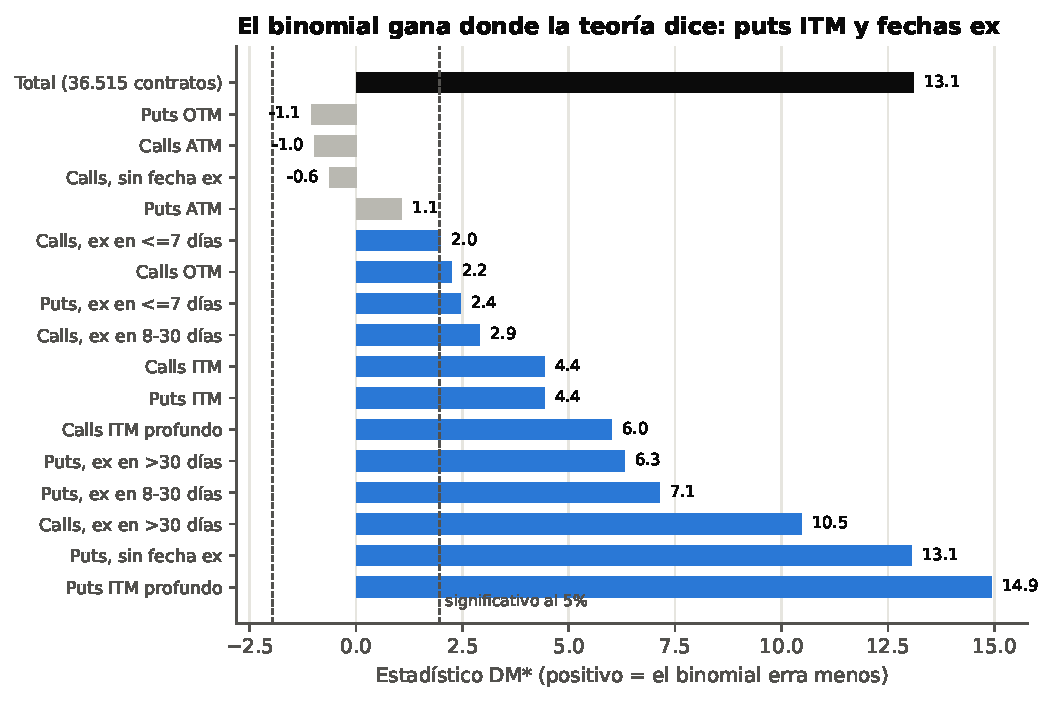
\includegraphics[width=0.84\linewidth]{figs/f04_dm_grupos.pdf}
\caption{Estadístico de Diebold-Mariano por tipo de contrato. Azul: el binomial erra significativamente menos. Gris:
no hay diferencia significativa.}
\end{figure}

\begin{enumerate}
\item \textbf{El binomial reprecia mejor}: $\bar d = 0{,}037$ medios spreads, $DM^* = 13{,}1$ ($p \approx 10^{-28}$).
\item \textbf{La diferencia está donde la teoría la pone}: puts muy dentro del dinero ($DM^* = 14{,}9$) y calls con
  una fecha ex en su vida ($DM^*$ entre 2,9 y 10,5).
\item \textbf{Donde no tiene que haber diferencia, no la hay}: calls sin fecha ex ($p = 0{,}53$) y opciones fuera del
  dinero.
\item \textbf{Pero es poca frente al spread}: la prima de ejercicio supera medio spread sólo en el 0,3\% de los
  contratos. El 98,1\% de los precios del binomial y el 97,6\% de los de Black-Scholes caen dentro del bid-ask.
\item \textbf{En las opciones que opera la estrategia sí pesa}: la diferencia entre modelos supera los \usd{10} por
  contrato en el 30\% de los casos. Black-Scholes valúa las puts dentro del dinero \usd{19} por contrato por debajo del
  mercado, y en la competencia eso lo empuja a venderlas baratas.
\end{enumerate}

\begin{criollo}
Los dos modelos cuentan casi la misma historia porque cada uno ajusta su volatilidad para parecerse al mercado. El
binomial gana donde tiene que ganar (puts profundas y dividendos), y gana con mucha confianza estadística, pero por
una diferencia que casi nunca cambia una decisión.
\end{criollo}

\subsection{Coberturas con griegas}

Experimento: se vende un contrato de cada opción del universo el primer día que aparece y se la sigue hasta 10
ruedas, cubriéndola cada día: 1.749 posiciones y 3.272 días-posición.

\begin{figure}[h]
\centering
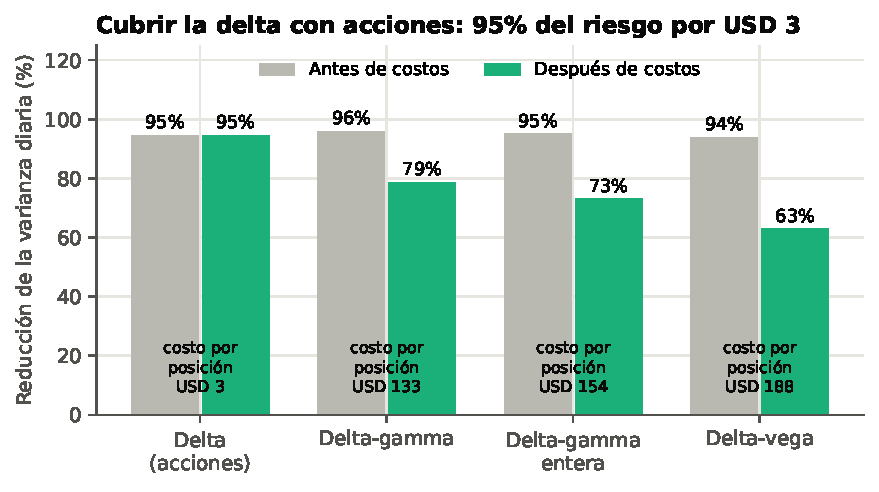
\includegraphics[width=0.84\linewidth]{figs/f05_coberturas.pdf}
\caption{Efectividad antes y después de costos (medio spread observado y \usd{0,65} por contrato en opciones, 1 punto
básico en acciones).}
\end{figure}

\begin{itemize}
\item \textbf{Delta con acciones es la mejor después de costos}: 95\% de efectividad por \usd{3} por posición.
\item \textbf{Cubrir la gamma no paga}: gana un punto antes de costos, pero armar y desarmar la opción de cobertura
  cuesta unos \usd{130} por posición. Neta, la delta-gamma queda en 79\% y la delta-vega en 63\%.
\item \textbf{Para cubrir, los dos modelos son equivalentes}: la delta difiere en 0,004 en promedio y Diebold-Mariano
  no encuentra diferencia ($p = 0{,}79$).
\item \textbf{Hace falta que los precios sean del mismo momento}: marcando la acción al cierre, la efectividad cae de
  95\% a 67\%. No falla la cobertura, falla el dato.
\end{itemize}

\subsection{Estrés por Monte Carlo}

Se estresa la cartera que el sistema abriría a capacidad máxima el 20 de noviembre (tres estructuras por modelo, en
BA y RTX), a 10 ruedas, con 5.000 trayectorias por escenario y las reglas de producción.

\begin{figure}[h]
\centering
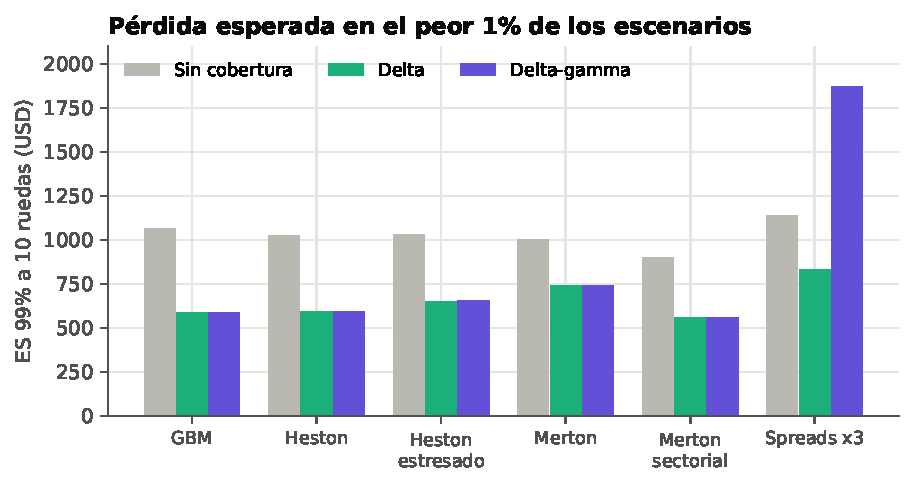
\includegraphics[width=0.86\linewidth]{figs/f06_estres.pdf}
\caption{Pérdida esperada en el peor 1\% de los escenarios (ES 99\%), al mid, para la cuenta completa.}
\end{figure}

\begin{itemize}
\item \textbf{La cobertura delta baja el riesgo de cola entre 25\% y 45\%} en todos los escenarios. La delta-gamma
  entera da lo mismo, porque la gamma de estas estructuras pide entre $-0{,}03$ y $0{,}06$ contratos, que redondean a
  0. Con spreads triples es peor, porque compra gamma pagando el spread.
\item \textbf{El riesgo dominante es la liquidez}: cerrar toda la cartera cruzando el spread cuesta \usd{708} en
  condiciones normales y \usd{2.443} con spreads triples, más que cualquier escenario de mercado.
\item \textbf{La pérdida está acotada}: ni una caída de 15\% en un día con la volatilidad 15 puntos arriba, ni la
  repetición del COVID o de los aranceles de 2025, disparan el corte por pérdida diaria. El kill-switch salta en el
  2\% a 6\% de las trayectorias.
\end{itemize}

\subsection{La decisión}

Los criterios se escribieron en \code{scripts/scorecard.py} \textbf{antes} de tener datos de paper. Modelo: gana el
que gana más criterios y, si empatan, Black-Scholes por ser el más simple. Cobertura: gana la que gana más
criterios y, si empatan, la más barata.

\begin{center}
\small
\begin{tabularx}{\linewidth}{@{}>{\sffamily}lX>{\sffamily\bfseries}l@{}}
\toprule
\textbf{Criterio} & \textbf{Evidencia} & \textbf{Ganador} \\
\midrule
M1. Repricing (Diebold-Mariano) & $\bar d = 0{,}037$, $DM^* = 13{,}1$ & \textcolor{crr}{binomial} \\
M2. Relevancia económica & la prima de ejercicio supera medio spread en el 0,3\% & empate \\
M3. Cobertura delta (Diebold-Mariano) & $p = 0{,}79$ & empate \\
M4. P\&L por estructura & paper: pendiente. Simulación 2020–2026: $z=-0{,}21$ & empate (simulación) \\
\midrule
E1. Efectividad neta & delta 95\%, delta-gamma entera 73\% & \textcolor{aqua!70!black}{delta} \\
E2. ES 99\% promedio & delta \usd{660}, delta-gamma \usd{835}, sin cubrir \usd{1.026} & \textcolor{aqua!70!black}{delta} \\
E3. Costo en GBM & delta y delta-gamma \usd{1,41} & empate \\
\bottomrule
\end{tabularx}
\end{center}

\begin{idea}[Resultado]
\textbf{Binomial y cobertura delta.} El binomial gana porque es el modelo correcto para opciones americanas con
dividendos discretos y los datos lo confirman. Pero hay que decirlo con su tamaño: rara vez cambia si un precio está
dentro del spread, no cambia la cobertura y, como muestra la sección siguiente, tampoco cambia el P\&L.
\end{idea}

\newpage
% ================================================================ 8. SIMULACIÓN HISTÓRICA
\section{Simulación histórica 2020–2026}

\subsection{Qué es y por qué la hicimos}

El paper trading en vivo tarda semanas en juntar operaciones. Para tener evidencia con más peso, hicimos correr
\textbf{el sistema completo de producción sobre siete años de datos reales}, foto por foto, como si hubiera estado
operando desde enero de 2020: los dos modelos compitiendo, el mismo cupo, las mismas órdenes maker, las mismas reglas
de riesgo y las mismas coberturas. Usa las mismas funciones que el robot en vivo.

\begin{minipage}[t]{0.235\linewidth}\kpi{1.229}{fotos diarias\\de la cadena}{crr}\end{minipage}\hfill
\begin{minipage}[t]{0.235\linewidth}\kpi{503.711}{cotizaciones\\(65\% operables)}{bsm}\end{minipage}\hfill
\begin{minipage}[t]{0.235\linewidth}\kpi{2.992}{órdenes\\publicadas}{violet}\end{minipage}\hfill
\begin{minipage}[t]{0.235\linewidth}\kpi{185}{estructuras\\cerradas}{aqua}\end{minipage}

\begin{ojo}[Por qué empieza en 2020 y no en 2019]
La base pública de opciones con bid y ask (DoltHub) arranca en enero de 2020. Entre 2020 y 2025 tiene fotos los
lunes, miércoles y viernes, y desde 2026 todos los días. Las opciones de RTX aparecen recién en abril de 2020 (antes
la empresa era UTX). Enero–marzo de 2020 tiene sólo BA y LMT, pero cubre el COVID.
\end{ojo}

\subsection{Resultado general}

\begin{figure}[h]
\centering
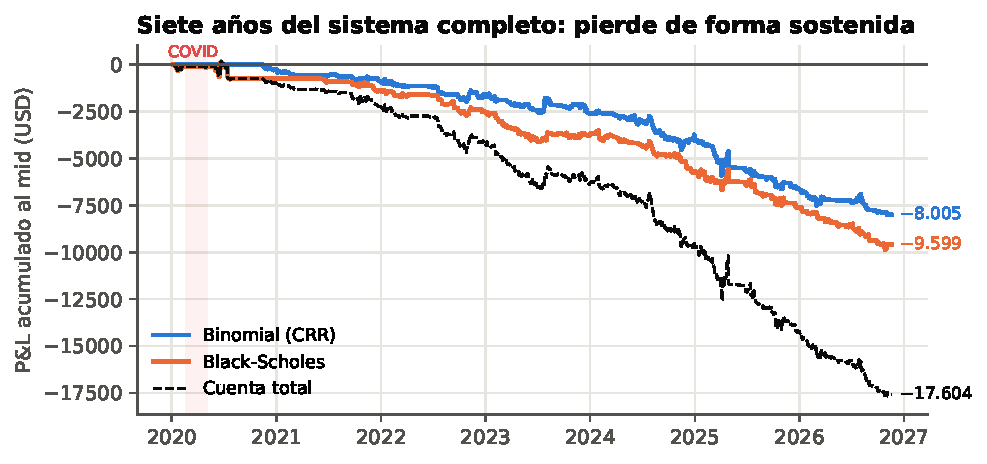
\includegraphics[width=0.9\linewidth]{figs/f07_replay_equity.pdf}
\caption{Valor acumulado de cada modelo y de la cuenta, al mid y con la cobertura delta incluida.}
\end{figure}

\begin{center}
\small
\begin{tabular}{@{}l>{\color{crr}}r>{\color{bsm}}r@{}}
\toprule
\sffamily\bfseries Con cobertura delta (producción) & \sffamily\bfseries\color{crr}Binomial & \sffamily\bfseries\color{bsm}Black-Scholes \\
\midrule
Órdenes publicadas & 1.498 & 1.494 \\
Llenadas & 86 (5,7\%) & 99 (6,6\%) \\
Estructuras cerradas & 86 & 99 \\
Con ganancia & 35\% & 44\% \\
P\&L realizado de las estructuras & \usd{−8.704} & \usd{−9.560} \\
P\&L medio por estructura (error estándar) & \usd{−101} (14) & \usd{−97} (17) \\
Valor final al mid, con la cobertura & \usd{−8.005} & \usd{−9.599} \\
Costo de la cobertura en siete años & \usd{23} & \usd{32} \\
Peor caída desde un máximo & \usd{−8.005} & \usd{−10.032} \\
\bottomrule
\end{tabular}
\end{center}

\begin{figure}[h]
\centering
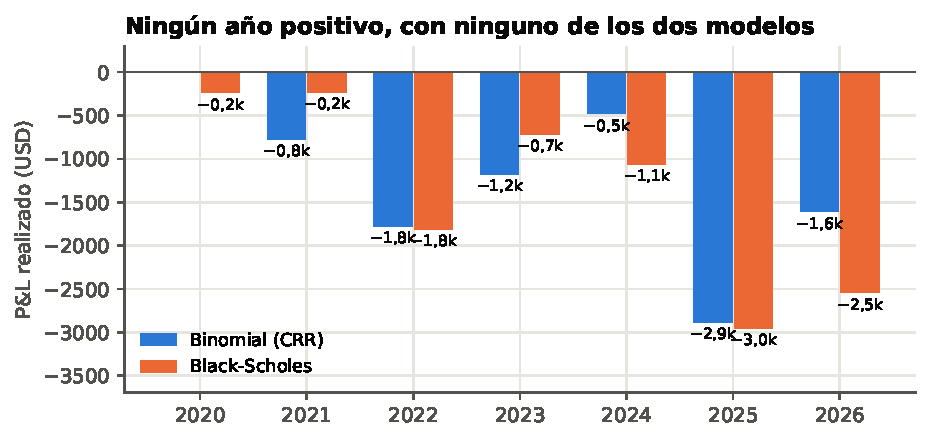
\includegraphics[width=0.9\linewidth]{figs/f08_replay_anios.pdf}
\caption{P\&L realizado por año de cierre. Valores en miles de dólares.}
\end{figure}

La pérdida no se concentra en una crisis: es \textbf{sostenida y pareja}. 2025 es el peor año para los dos modelos.
Por subyacente, BA concentra 142 de las 185 estructuras (\usd{−12.251}), porque es el que tiene más contratos dentro
de los filtros; RTX suma 32 (\usd{−4.002}) y LMT 11 (\usd{−2.011}).

\subsection{Por qué pierde: la selección adversa}

\begin{figure}[h]
\centering
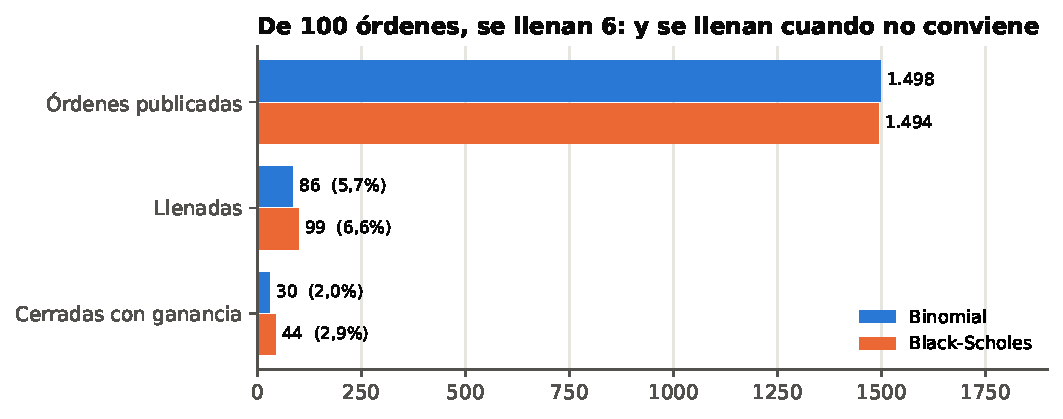
\includegraphics[width=0.88\linewidth]{figs/f09_replay_embudo.pdf}
\caption{De casi 3.000 órdenes, se llenan 185.}
\end{figure}

\begin{figure}[h]
\centering
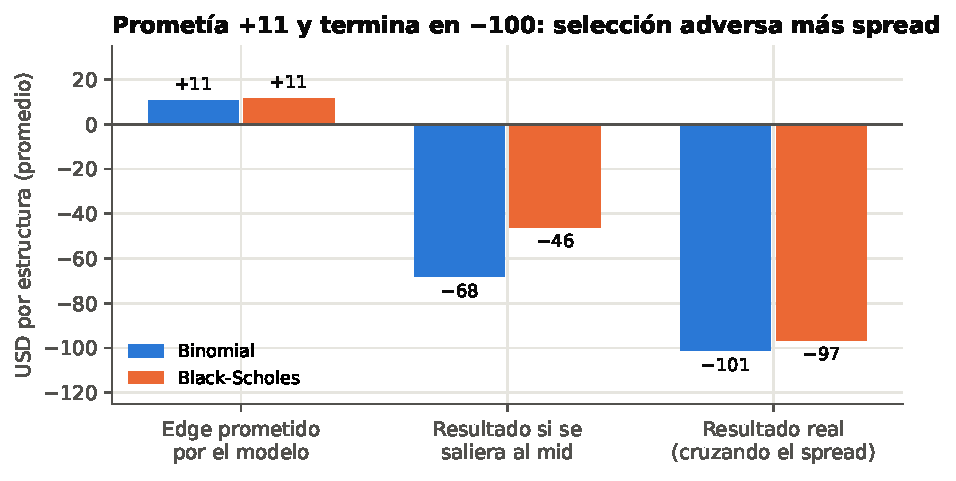
\includegraphics[width=0.88\linewidth]{figs/f10_replay_descomposicion.pdf}
\caption{Promedio por estructura cerrada: el edge que prometía el modelo al publicar la orden, el resultado si se
pudiera salir al mid y el resultado real, pagando el spread de salida.}
\end{figure}

La figura anterior es la más importante del trabajo. Cuenta tres cosas:

\begin{enumerate}
\item \textbf{El modelo promete +\usd{11}} por estructura. Es lo que se pide para publicar la orden.
\item \textbf{Aun saliendo al mid, se pierden entre \usd{46} y 68.} Es la selección adversa (Glosten y Milgrom, 1985):
  una orden pasiva al precio del modelo se llena justo cuando el mercado la atraviesa, es decir, cuando llegó
  información nueva que el modelo, calibrado en la foto anterior, todavía no incorporó. El edge existe en el momento
  del llenado, pero contra un precio viejo.
\item \textbf{Pagar el spread de salida suma otros \usd{33} a 50 de pérdida.} Con spreads de 14\% en la mediana,
  entrar y salir es caro.
\end{enumerate}

\begin{criollo}
Es como poner un cartel de ``compro dólares a 1.000'' cuando el modelo dice que valen 1.010. Si alguien te los vende
a 1.000, probablemente sea porque ya sabe que bajaron a 980. Te llenan justo cuando no te conviene.
\end{criollo}

\subsection{Cómo terminan las posiciones}

\begin{figure}[h]
\centering
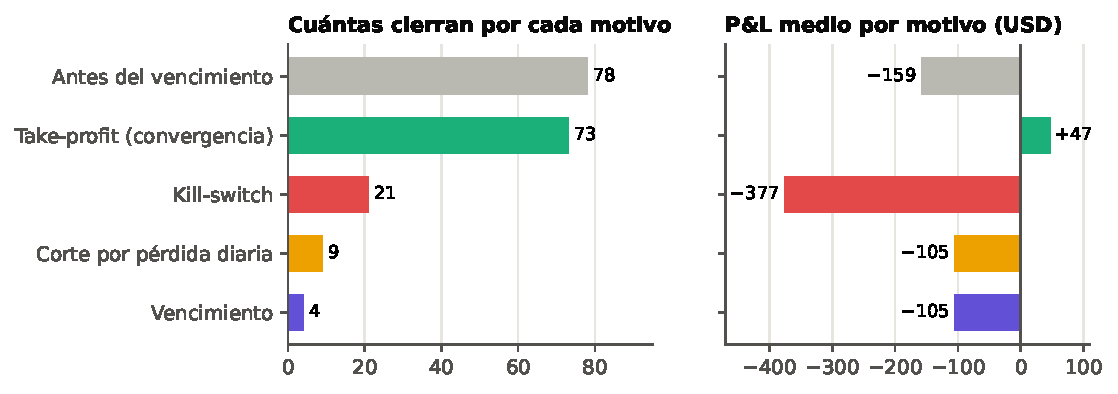
\includegraphics[width=0.92\linewidth]{figs/f11_replay_motivos.pdf}
\caption{Motivo de cierre de las 185 estructuras y P\&L medio de cada grupo.}
\end{figure}

\begin{itemize}
\item \textbf{73 cierran por take-profit}, con \usd{+47} de promedio: cuando el modelo tiene razón, gana.
\item \textbf{78 llegan a 2 días del vencimiento sin converger} y se cierran con \usd{−159} de promedio.
\item \textbf{21 tocan el kill-switch}, con \usd{−377}: el corte se mide al mid y el cierre efectivo paga el spread.
\item El corte por pérdida diaria de la cuenta se activó en 2 días de siete años (agosto de 2024 y abril de 2025).
\end{itemize}

\begin{figure}[h]
\centering
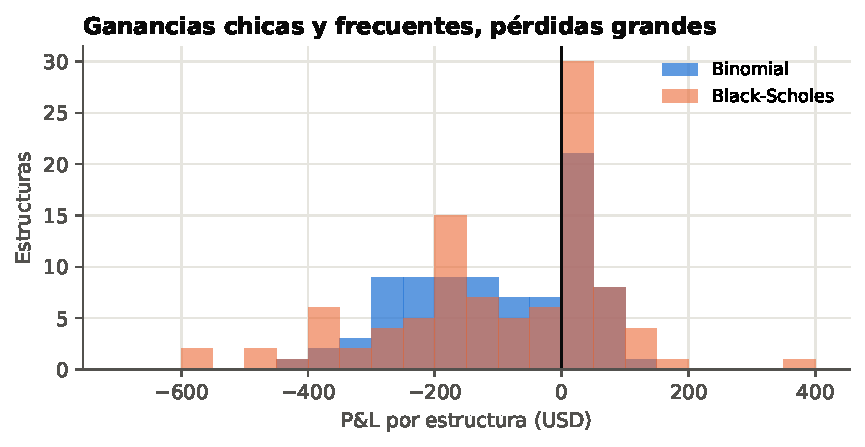
\includegraphics[width=0.84\linewidth]{figs/f12_replay_distribucion.pdf}
\caption{Distribución del P\&L por estructura. El perfil es el de vender seguros baratos: muchas ganancias chicas y
algunas pérdidas grandes.}
\end{figure}

\subsection{Binomial contra Black-Scholes en P\&L (criterio M4)}

\begin{figure}[h]
\centering
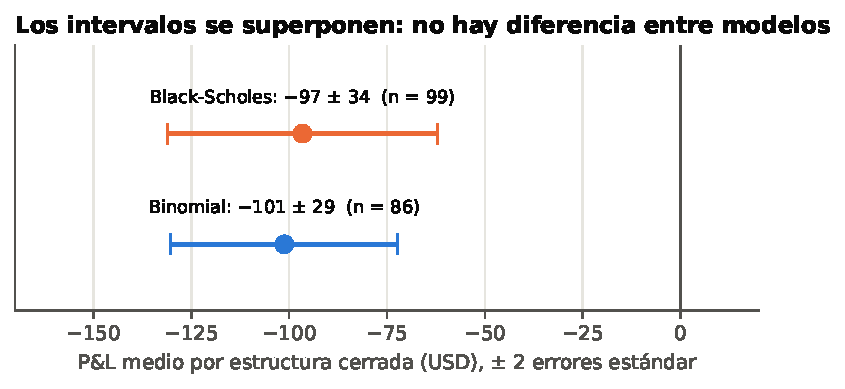
\includegraphics[width=0.8\linewidth]{figs/f13_replay_m4.pdf}
\caption{P\&L medio por estructura con un intervalo de dos errores estándar.}
\end{figure}

\begin{formula}
\[
\bar\pi_{CRR} - \bar\pi_{BS} = -101{,}2 - (-96{,}6) = -4{,}6, \qquad
EE = \sqrt{\frac{s^2_{CRR}}{n_{CRR}} + \frac{s^2_{BS}}{n_{BS}}} = 22{,}5, \qquad z = -0{,}21 .
\]
\end{formula}

Se cumple el mínimo de 10 estructuras por modelo, pero la diferencia no supera dos errores estándar: \textbf{empate}.
Es coherente con todo lo anterior: los dos modelos ven casi lo mismo y los dos pierden por la misma razón.

\subsection{Con y sin cobertura}

\begin{center}
\small
\begin{tabular}{@{}lrrrr@{}}
\toprule
 & \multicolumn{2}{c}{\sffamily\bfseries\color{crr}Binomial} & \multicolumn{2}{c}{\sffamily\bfseries\color{bsm}Black-Scholes} \\
\cmidrule(lr){2-3}\cmidrule(l){4-5}
\sffamily\bfseries Modo & Cerradas & Valor final al mid & Cerradas & Valor final al mid \\
\midrule
Sin cobertura & 90 & \usd{−10.861} & 95 & \usd{−8.919} \\
Delta & 86 & \usd{−8.005} & 99 & \usd{−9.599} \\
Delta-gamma & 86 & \usd{−8.005} & 99 & \usd{−9.599} \\
\bottomrule
\end{tabular}
\end{center}

\begin{itemize}
\item \textbf{La cobertura delta cuesta casi nada} (\usd{23} y \usd{32} en siete años) y cambia poco el resultado: las
  verticales de una unidad tienen delta chica y la estrategia pierde por precio, no por movimientos de la acción.
\item \textbf{La delta-gamma da exactamente lo mismo que la delta} porque nunca llega a comprar la opción de
  cobertura: el cociente $-\Gamma_{\text{libro}}/(100\,\Gamma_{\text{ATM}})$ queda casi siempre debajo de 0,05 y
  redondea a 0 contratos. No es un error: pasa lo mismo en vivo con este tamaño de posición.
\item Los modos no son idénticos en cantidad de operaciones porque las reglas de riesgo interactúan con la cobertura
  (un corte por pérdida diaria cierra todo y libera cupo en días distintos).
\end{itemize}

\begin{ojo}[Lo que hay que aclarar al presentar estos números]
Entre 2020 y 2025 hay fotos sólo lunes, miércoles y viernes: una orden se llena (o no) dos o tres días después, lo
que es más conservador que la realidad, donde puede llenarse en cualquier momento del día. Las comisiones son las
de Alpaca (\usd{0,65} por contrato) y no hay costo de préstamo ni de margen. Y los dividendos de BA se cortaron en
marzo de 2020: el modelo lo toma con las fechas de anuncio.
\end{ojo}

\newpage
% ================================================================ 9. DÓNDE CORRE
\section{Dónde corre}

El sistema opera solo en una máquina virtual de \textbf{Oracle Cloud}, dentro del plan \emph{Always Free}, contra la
cuenta \emph{paper} (de prueba, sin plata real) de \textbf{Alpaca}. No depende de que ninguna computadora del grupo
esté prendida.

\begin{figure}[h]
\centering
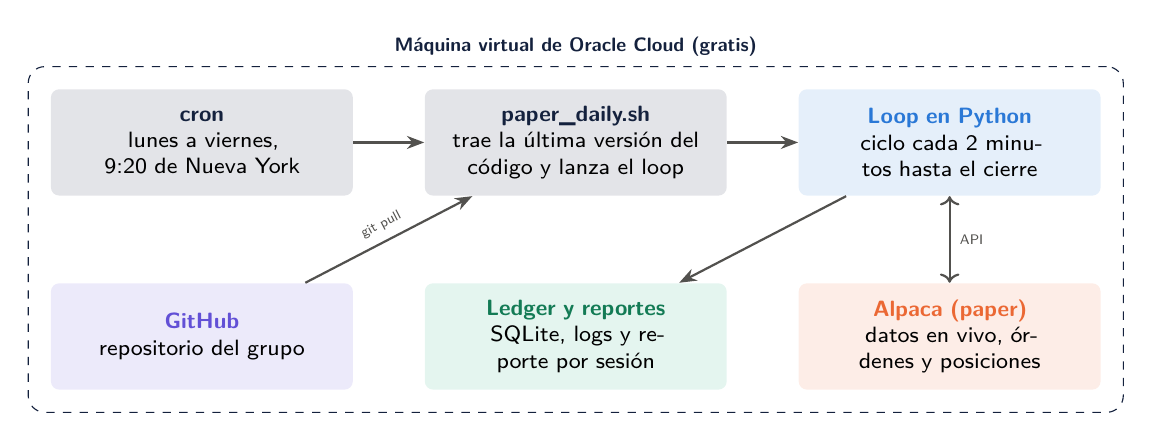
\begin{tikzpicture}[
  node distance=0.6cm and 0.9cm,
  box/.style={draw=none,fill=#1!12,rounded corners=3pt,minimum height=1.35cm,text width=3.6cm,align=center,
              font=\sffamily\footnotesize},
  arr/.style={-{Stealth[length=2.2mm]},thick,color=ink2},
  lab/.style={font=\sffamily\tiny,text=ink2,midway}]
\node[box=navy] (cron) {{\bfseries\color{navy}cron}\\ lunes a viernes, 9:20 de Nueva York};
\node[box=navy,right=of cron] (sh) {{\bfseries\color{navy}paper\_daily.sh}\\ trae la última versión del código y lanza el loop};
\node[box=crr,right=of sh] (py) {{\bfseries\color{crr}Loop en Python}\\ ciclo cada 2 minutos hasta el cierre};
\node[box=bsm,below=1.1cm of py] (alp) {{\bfseries\color{bsm}Alpaca (paper)}\\ datos en vivo, órdenes y posiciones};
\node[box=aqua,below=1.1cm of sh] (led) {{\bfseries\color{aqua!70!black}Ledger y reportes}\\ SQLite, logs y reporte por sesión};
\node[box=violet,below=1.1cm of cron] (gh) {{\bfseries\color{violet}GitHub}\\ repositorio del grupo};
\begin{scope}[on background layer]
\node[draw=navy,dashed,rounded corners=6pt,inner sep=8pt,fit=(cron)(sh)(py)(led),
      label={[font=\sffamily\scriptsize\bfseries,text=navy]above:Máquina virtual de Oracle Cloud (gratis)}] {};
\end{scope}
\draw[arr] (cron) -- (sh);
\draw[arr] (sh) -- (py);
\draw[arr,<->] (py) -- node[lab,right]{API} (alp);
\draw[arr] (py) -- (led);
\draw[arr] (gh) -- node[lab,above,sloped]{git pull} (sh);
\end{tikzpicture}
\caption{Arquitectura de producción.}
\end{figure}

\subsection{Cómo funciona un día}

\begin{enumerate}
\item A las \textbf{9:20 de Nueva York} (11:20 en Buenos Aires mientras rija la diferencia de 2 horas) el programador
  de tareas (\code{cron}) lanza el script.
\item El script baja la última versión del código de GitHub, se asegura de que no haya otra corrida en curso y arranca
  el loop con la configuración de producción.
\item El loop espera la apertura (9:30), opera y monitorea cada 2 minutos y termina después del cierre (16:00).
\item Queda el log del día y el reporte de la sesión con órdenes, llenados, griegas de cada libro y P\&L.
\end{enumerate}

\subsection{La máquina}

\begin{center}
\small
\begin{tabular}{@{}>{\sffamily}ll@{}}
\toprule
Proveedor & Oracle Cloud Infrastructure, región US East (Ashburn) \\
Tipo & VM.Standard.E2.1.Micro (\emph{Always Free}): 1 GB de RAM + 2 GB de swap \\
Sistema & Ubuntu 24.04, Python 3.12 \\
Costo & \usd{0}: se usan sólo recursos \emph{Always Free} y la cuenta no se pasó a pago \\
Instalación & un script (\code{deploy/oracle/setup_vm.sh}) instala todo y corre los 184 tests \\
Seguridad & las claves de Alpaca viven sólo en un archivo \code{.env} de la máquina, fuera del repositorio \\
\bottomrule
\end{tabular}
\end{center}

\subsection{Cómo se controla}

\begin{itemize}
\item \textbf{Ver cómo va}: conectarse por SSH y leer el log del día (\code{reportes/paper/logs/}).
\item \textbf{Cortar todo}: crear el archivo \code{KILL}; en el ciclo siguiente se cierran todas las posiciones.
\item \textbf{Traer los resultados}: el script \code{traer_resultados.ps1} copia reportes y ledger a una computadora.
\item \textbf{Riesgo operativo}: Oracle puede apagar una máquina gratuita que considere ociosa siete días seguidos. Se
  vuelve a prender desde la consola y la programación sigue igual.
\end{itemize}

% ================================================================ 10. ESTADO DEL PAPER
\section{Estado del paper trading y lo que falta}

\begin{itemize}
\item \textbf{En marcha desde el 23 de noviembre de 2026}, con la configuración completa de producción: los dos
  modelos compitiendo, cobertura delta-gamma, kill-switch de \usd{250} y corte diario de \usd{1.000}.
\item \textbf{Qué mide}: la tasa de llenado real (con órdenes que pueden llenarse en cualquier momento del día, no sólo
  en una foto), la selección adversa en producción, el costo real de la cobertura con llenados de verdad y el P\&L por
  modelo.
\item \textbf{Qué completa}: el criterio M4 \emph{en vivo}, que necesita al menos 10 estructuras cerradas por modelo.
  Con 2–3 semanas de ruedas debería alcanzar. El script \code{scorecard.py} lo evalúa directamente desde el ledger.
\item \textbf{Qué esperamos}: por la Parte 1 y la simulación histórica, que la estrategia pierda. La consigna no evalúa
  el retorno: el objetivo del paper es medir en producción lo que el backtest no puede ver.
\end{itemize}

\newpage
% ================================================================ 11. LIMITACIONES
\section{Limitaciones}

\begin{center}
\small
\renewcommand{\arraystretch}{1.25}
\begin{tabularx}{\linewidth}{@{}>{\sffamily\bfseries\raggedright\arraybackslash}p{4.1cm}X@{}}
\toprule
Limitación & Qué implica \\
\midrule
Una foto por día, sin hora documentada & El desfase con el cierre se mide y se absorbe con el spot implícito, pero no se elimina. El modelo de llenado ve un solo precio por día. \\
Fotos lunes, miércoles y viernes hasta 2025 & En la simulación, una orden se resuelve 2–3 días después: el llenado es más conservador que en la realidad. \\
Historia desde 2020 & DoltHub no tiene datos anteriores; RTX recién desde abril de 2020. \\
Sin volumen ni open interest & La liquidez se juzga sólo por el spread. \\
Pocas operaciones & 185 estructuras en siete años: alcanza para descartar una diferencia grande entre modelos, no una chica. \\
Coberturas en corridas cortas & DoltHub no trae todos los vencimientos todos los días (1,9 días por corrida): el costo de armar y desarmar pesa más que en una tenencia larga. \\
Supuestos del estrés & El mispricing no converge, la volatilidad se mueve en paralelo en toda la sonrisa y, en los escenarios históricos, la respuesta de la volatilidad es una regla. \\
Paper de Alpaca & No simula slippage, impacto, dividendos ni costo de préstamo, y el feed gratuito llega demorado. \\
Asignación anticipada & El detector de paridad la cubre con el peor caso, pero el backtest no la simula. \\
Supervivencia & Los subyacentes se eligieron hoy. Los tres siguen listados y RTX nace en abril de 2020 de la fusión de UTX con Raytheon: el sesgo es chico, pero existe. \\
\bottomrule
\end{tabularx}
\end{center}

% ================================================================ 12. PREGUNTAS
\section{Preguntas probables y cómo responderlas}

\newcommand{\pregunta}[2]{%
\begin{tcolorbox}[enhanced,breakable,colback=white,colframe=crr!30,boxrule=0.6pt,arc=3pt,left=9pt,right=9pt,top=5pt,bottom=5pt,before skip=6pt,after skip=6pt]
{\sffamily\bfseries\color{navy}#1}\par\vspace{3pt}#2
\end{tcolorbox}}

\pregunta{¿Por qué la estrategia pierde si el modelo dice que hay edge?}
{Porque el edge se mide contra un precio viejo. La orden límite queda quieta al precio del modelo y sólo se llena
cuando el mercado la atraviesa, es decir, cuando hay información nueva. Es selección adversa (Glosten y Milgrom,
1985). En la simulación histórica, el modelo prometía \usd{+11} por estructura y, saliendo al mid, el resultado fue de
\usd{−46} a −68.}

\pregunta{Entonces, ¿el binomial no sirve?}
{Sirve para valuar y cubrir: reproduce el 98\% de los precios dentro del bid-ask y gana a Black-Scholes donde la
teoría dice (puts ITM, fechas ex). Lo que no hace es generar plata por sí solo con órdenes pasivas: valuar bien no
alcanza para ganarle al spread.}

\pregunta{¿Por qué en la Parte 1 ganaban USD 19.055 y ahora no hay arbitraje?}
{Porque el bid y el ask eran sintéticos y la foto y el cierre no eran del mismo momento. Con precios reales y
sincronizados, las 1.744 violaciones de paridad bajan a 3 y ninguna se puede ejecutar. Es lo esperable en un mercado
de opciones listadas con spreads de 14–18\%.}

\pregunta{¿Por qué Black-Scholes y el binomial dan casi lo mismo?}
{Porque cada uno calibra su propia sonrisa: la diferencia entre la valuación americana y la europea se absorbe casi
entera en la volatilidad ajustada. Sólo queda donde el ejercicio anticipado vale mucho, y ahí el binomial gana.}

\pregunta{La consigna pide coberturas con griegas. ¿Por qué recomiendan sólo delta?}
{Porque probamos las cuatro y, después de costos, la delta es la mejor: 95\% contra 63–79\%. Igual, en producción corre
la delta-gamma para medir su costo con llenados reales. Con posiciones de una unidad, la gamma pide menos de un
contrato y redondea a cero.}

\pregunta{¿Cómo evitaron el lookahead?}
{Cada señal de una foto se ejecuta contra la foto siguiente. Los dividendos entran recién cuando se declaran. La
calibración usa sólo datos del día. En el walk-forward, las posiciones de calibración se cierran al final de su
ventana y ninguna cruza al período de evaluación.}

\pregunta{¿Qué tan realista es el modelo de llenado?}
{Es conservador: con una foto por día sólo vemos un precio, y una orden real puede llenarse con cualquier cruce
durante la rueda. El paper trading mide justamente la tasa de llenado real.}

\pregunta{¿Por qué el kill-switch se mide al mid y el take-profit a liquidación?}
{Medido a liquidación, el kill-switch se disparaba al abrir cada posición sólo por el spread. El take-profit sí se
mide a liquidación porque esa ganancia hay que poder cobrarla pagando el spread.}

\pregunta{¿Por qué la simulación empieza en 2020?}
{Es lo máximo que permite la única fuente pública de bid y ask de opciones (DoltHub). Igual cubre el COVID, la guerra
en Ucrania, la suba de tasas de 2022 y los aranceles de 2025.}

\pregunta{¿Qué cambiarían para que gane?}
{Operar sólo cuando el desvío contra el modelo supere el spread entero (tomar liquidez en vez de darla), reaccionar
más rápido para que el modelo no quede desactualizado, o ir a estrategias de volatilidad con horizonte más largo,
donde el costo de entrar y salir pese menos.}

\newpage
% ================================================================ 13. GLOSARIO
\section{Glosario}

\begin{multicols}{2}
\small
\begin{description}[leftmargin=0pt,style=nextline,itemsep=0.4em,font=\sffamily\bfseries\color{navy}]
\item[Arbitraje] Ganancia sin riesgo por una inconsistencia de precios. No depende de ningún modelo.
\item[Bid / ask] Precio al que el mercado compra / vende. El \emph{mid} es el promedio; el \emph{spread}, la diferencia.
\item[Butterfly] Comprar un strike bajo, vender dos del medio y comprar uno alto. Pérdida máxima acotada.
\item[Calibrar] Ajustar los parámetros del modelo (la sonrisa) para que sus precios se parezcan a los del mercado.
\item[CRR] Árbol binomial de Cox, Ross y Rubinstein. Valúa opciones americanas.
\item[Delta-gamma] Cobertura con acciones (delta) y con otra opción (gamma).
\item[Diebold-Mariano] Test estadístico para decidir cuál de dos modelos erra menos.
\item[Dividendo escrowed] Modelo que separa el precio en una parte riesgosa y el valor presente de los dividendos.
\item[Edge] Diferencia entre el valor del modelo y el precio pagado, neta de comisiones.
\item[EEP] Prima de ejercicio anticipado: lo que vale poder ejercer antes del vencimiento.
\item[ES 99\%] \emph{Expected shortfall}: pérdida promedio en el peor 1\% de los escenarios.
\item[Fecha ex] Primer día en que la acción cotiza sin el derecho al dividendo.
\item[ITM / ATM / OTM] Dentro, en y fuera del dinero.
\item[Kill-switch] Corte automático de una posición cuando pierde demasiado.
\item[Ledger] Registro propio de órdenes y posiciones, que se compara con el del broker.
\item[Lookahead] Usar en una decisión información que todavía no se conocía. Invalida un backtest.
\item[Maker / taker] Orden que espera en el libro (da liquidez) / que cruza el spread (toma liquidez).
\item[Paper trading] Operar con plata ficticia contra el mercado real.
\item[Paridad put-call] Relación entre call, put, acción y bono que no se puede violar sin arbitraje.
\item[Selección adversa] Que te llenen la orden justo cuando la contraparte sabe algo que vos no.
\item[Sharpe deflactado] Sharpe corregido por la cantidad de configuraciones probadas.
\item[Sonrisa (smile/skew)] Forma de la volatilidad implícita según el strike.
\item[Spot implícito] Precio de la acción deducido de la propia cadena de opciones con la paridad.
\item[Vertical] Comprar un strike y vender otro del mismo vencimiento. Pérdida máxima acotada.
\item[Volatilidad implícita] La $\sigma$ que hace que el modelo dé el precio de mercado.
\item[Walk-forward] Calibrar con el pasado y evaluar en el período siguiente, avanzando en el tiempo.
\end{description}
\end{multicols}

\newpage
% ================================================================ 14. FUENTES
\section{Fuentes de datos, herramientas y uso de IA}

\subsection{Datos}

\begin{center}
\small
\begin{tabularx}{\linewidth}{@{}>{\sffamily\bfseries}lX@{}}
\toprule
Fuente & Qué aporta \\
\midrule
DoltHub (\code{post-no-preference/options}) & Foto diaria de la cadena con bid, ask, IV y griegas del proveedor. 2026 para el análisis principal; 2020–2026 para la simulación histórica. \\
Alpaca (cuenta paper) & Datos en vivo, universo de contratos, órdenes multipata y posiciones. Comisión supuesta: \usd{0,65} por contrato. \\
Yahoo Finance & Cierres sin ajustar, 10 años de historia para el estrés, dividendos y la tasa a 13 semanas (\^{}IRX). \\
Polygon & Dividendos con fecha de declaración, para usarlos \emph{point-in-time}. \\
Oracle Cloud & Máquina virtual gratuita donde corre el paper trading. \\
\bottomrule
\end{tabularx}
\end{center}

\subsection{Herramientas}

Python 3.12 (pandas, NumPy, SciPy, alpaca-py, matplotlib), pytest para los 184 tests, SQLite para el ledger, Git y
GitHub para el código, y \LaTeX{} para este documento.

\subsection{Uso de inteligencia artificial}

Usamos \textbf{Claude} (Anthropic), uno de los modelos permitidos. El registro completo de cada interacción (el
pedido, la respuesta y por qué se delegó) está en \code{AI_LOG.md}, en la raíz del repositorio.

\begin{itemize}
\item \textbf{Delegamos}: escribir y testear código, auditar el código heredado y el de la cátedra, descargar y curar
  datos, y escribir documentación técnica, siempre con tests que fijan el comportamiento esperado.
\item \textbf{No delegamos}: la elección de subyacentes, la grilla de parámetros (declarada antes de ver resultados),
  los criterios de decisión ni la lectura de los resultados. Cada número sale de un script del repositorio, no de una
  respuesta del chat.
\end{itemize}

\subsection{Bibliografía}

\small
\begin{itemize}[leftmargin=1em]
\item Black, F. y Scholes, M. (1973). The Pricing of Options and Corporate Liabilities. \emph{JPE}.
\item Merton, R. (1973). Theory of Rational Option Pricing. \emph{Bell Journal of Economics}.
\item Cox, J., Ross, S. y Rubinstein, M. (1979). Option Pricing: A Simplified Approach. \emph{JFE}.
\item Hull, J. \emph{Options, Futures, and Other Derivatives}, cap. 21 (dividendos discretos).
\item Heston, S. (1993). A Closed-Form Solution for Options with Stochastic Volatility. \emph{RFS}.
\item Merton, R. (1976). Option Pricing When Underlying Stock Returns Are Discontinuous. \emph{JFE}.
\item Lord, R., Koekkoek, R. y van Dijk, D. (2010). A Comparison of Biased Simulation Schemes for Stochastic Volatility Models. \emph{Quantitative Finance}.
\item Diebold, F. y Mariano, R. (1995). Comparing Predictive Accuracy. \emph{JBES}; Harvey, Leybourne y Newbold (1997); Newey y West (1987).
\item Glosten, L. y Milgrom, P. (1985). Bid, Ask and Transaction Prices in a Specialist Market. \emph{JFE}.
\item Leland, H. (1985). Option Pricing and Replication with Transactions Costs. \emph{Journal of Finance}.
\item Bailey, D. y López de Prado, M. (2014). The Deflated Sharpe Ratio. \emph{JPM}.
\item Gatheral, J. (2006). \emph{The Volatility Surface}. Wiley.
\item Ofek, E., Richardson, M. y Whitelaw, R. (2004). Limited Arbitrage and Short Sales Restrictions. \emph{JFE}.
\end{itemize}

\end{document}
